\documentclass{standalone}
\usepackage{tikz}
\usepackage{ctex,siunitx}
\setCJKmainfont{Noto Serif CJK SC}
\usepackage{tkz-euclide}
\usepackage{amsmath}
\usepackage{wasysym}
\usetikzlibrary{patterns, calc}
\usetikzlibrary {decorations.pathmorphing, decorations.pathreplacing, decorations.shapes,}
\begin{document}
\small
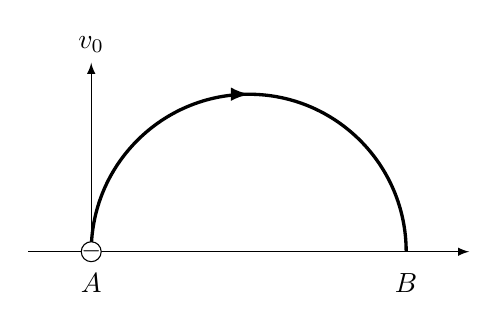
\begin{tikzpicture}[>=latex,scale=0.8]
  \draw[->] (-1,0)--(6,0);
  \draw[->] (0,0)--(0,3)node [above]{$v_0$};
  \draw[very thick,postaction={decorate},decoration={markings,mark={at position 0.5 with {\arrow{>}}}}] (0,0) arc (180:0:2.5); 
  \node at (0,-.5){$A$};\node at (5,-.5){$B$};
  \draw (0,0) [fill=white]circle (4.5pt);
  \node at  (0,0) {\small $-$};
\end{tikzpicture}
\end{document}